\begin{frame}
  \frametitle{Impieghi}

  \begin{itemize}
   \item<1-> Impieghi:
   \begin{itemize}
    \item<2-> Criptomonete
    \item<3-> Pubblica amministrazione
    \item<4-> \textit{Internet of Things}
    % TODO potrei cambiare e mettere il servizio di chat - o potrei rimuoverlo
    \item<5-> Salvataggio dati
    \item<6-> Autenticazione \& autorizzazione
   \end{itemize}
  \end{itemize}

 \begin{textblock*}{5cm}(8cm,2.5cm)
  
\includegraphics[scale=0.3]{bagOfMoney}
 \end{textblock*}

 \begin{textblock*}{5cm}(7.5cm,5.5cm)
  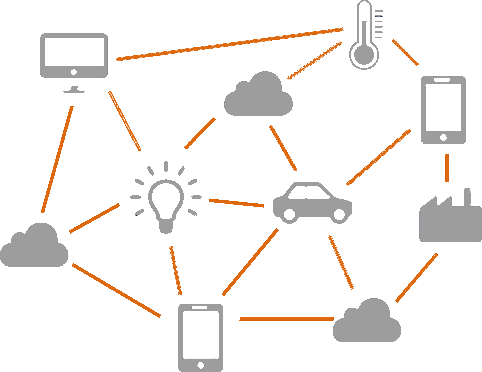
\includegraphics[scale=0.2]{IoT}
 \end{textblock*}

 \begin{textblock*}{5cm}(5cm,1.5cm)
  
\includegraphics[scale=0.1]{file}
 \end{textblock*}


\end{frame}
